\documentclass[11pt]{article}

\usepackage[utf8]{inputenc}
\usepackage[margin=1.25in]{geometry}
\usepackage{subcaption}
\usepackage{cite}
\usepackage{graphicx}
\usepackage[hidelinks]{hyperref}
\usepackage{amssymb}
\usepackage{amsmath}
\usepackage{caption} % For captioning tables and figures
\usepackage{array} % For more flexible table formatting


\begin{document}

\begin{titlepage}
	\centering
	
\includegraphics[width=0.2\textwidth]{assets/uni-logo.png}\par\vspace{0.5cm}
	{\scshape\LARGE Friedrich Schiller University, Jena \par}
	\vspace{1cm}
	{\scshape\Large Seminar Paper for Advanced Methods in Computer Vision\par}
	\vspace{1.5cm}
	{\huge\bfseries An overview over image generating artificial intelligence (TODO!!!)\par}
	\vspace{2cm}
	{\Large\itshape Phillip Rothenbeck, Lean Manthey, and Moritz Seppelt\par}
	\vfill
	supervised by\par
	M.Sc.~Niklas \textsc{Penzel}

	\vfill

	{\large \today\par}
\end{titlepage}

\tableofcontents
\newpage

\section{Introduction}
1 Seite

\section{Related Work}
1 - 2 Seiten. Einfach nur related work von Papern abschreiben
\section{Background}
\subsection{Stable Diffusion}
In the beginning of 2022, computer scientists from LMU Munich and IWR Heidelberg proposed an improved approach on how to achieve high-resolution image synthesis\cite{rombach2022stablediffusion}. They coined this method “latent diffusion models”. It introduced the necessary performance boost to make productively using and training image models really feasible. Diffusion models were known before. The new idea was to not generate the full image using iterative diffusion but to generate a low-dimensional representation of that image first using denoising and then to upscale it. This small change was enough to accomplish the required performance boost. Later this model was called “Stable Diffusion”.

In this chapter, we will provide an overview of the inner working of stable diffusion and thereby focus on the text-to-image procedure. Later we will also demonstrate how this can be extended to also implement e.g. in-painting. It mainly consists of three parts:
\begin{enumerate}
    \item The text input is converted to conditioning vectors. This is done using a transformer architecture.
    \item The main step is the iterative denoising. Here the conditioning vectors will influence the resulting latent representation. A neural network in the U-net architecture does the heavy lifting.
    \item Finally, the latent representation must be converted into the final image. For that, an auto decoder is used. 
\end{enumerate}

First let's assume, all the machine learning components have already their trained weights and biases. Equipped with these, we will go through step by step how a text-input is turned into an image. Afterwards, the training process is presented.

\subsubsection{Conditioning}
For stable diffusion, the conditioning process is just a series of different existing components plugged together with the goal of semantically understanding the input prompt. First the input sentence gets tokenized. They were using the BERT-Tokenizer\cite{devlin2019bert}. The result of this step is a sequence of tokens, which can be thought of words or part of words. 

Secondly, these tokens get embedded into some Euclidean vector space. Here already some semantic meaning gets encoded. Tokens that have similar meanings will be mapped to vectors that point to approximately the same region in this high-dimensional space. For example the words “achieve” and “accomplish” would be closer than “achieve” and “annoying”. But even more, direction or distances can also be interpretable already. This could be thought of as relations between words. For example, it is expectable that the embedding of “Germany” and “Berlin” have the same distance as “Spain” and “Madrid”. 

It operates by computing three different vectors for each token in the input sequence for each type of relationship there could be in the sentence: the Query ($Q$), the Key ($K$), and the Value ($V$) vectors. These vectors are derived from the embedded token vectors through linear transformations, which are essentially matrix multiplications with learned weight matrices. Specifically, for each token, we calculate:
$$Q = X \cdot W_Q,\quad K = X\cdot W_K,\quad V = X \cdot W_V$$
Where $X$ is the matrix of embedded token vectors, and $W_Q$, $W_K$ and $W_V$ are learned weight matrices for the Query, Key, and Value, respectively.

Once we have the Query ($Q$), Key ($K$), and Value ($V$) vectors for each token, the next step is to determine how much each token should focus on the others. The goal here is to figure out which other words in the sentence are most relevant to the current word, given the context.
Imagine each Query vector as a question that each word is asking about its context. The Key vectors, on the other hand, represent the possible answers that other words can provide. The dot product between a Query and a Key is like measuring how well the question matches the answer. If the Query and Key vectors are similar, it means that the word being asked about is highly relevant to the current word, and so it should be paid more attention.
However, to prevent these dot products from getting too large when working with high-dimensional vectors, we scale them down by the square root of the Key vector's dimension, $\sqrt{d_k}$.

$$\frac{QK^\top}{\sqrt{d_k}}$$

Next, we convert these scaled dot products into attention scores using a softmax function. The softmax function turns these scores into probabilities, where higher scores mean more attention should be given to that token. For example, if "Harry" is the current word, and its Query vector strongly matches the Key vector of "wizard", the attention mechanism will assign a high probability to "wizard", meaning that "Harry" will focus more on "wizard" in this context.

$$\mathrm{Attention Weights} = \mathrm{softmax}\left(\frac{QK^\top}{\sqrt{d_k}}\right)$$

Finally, these attention scores are used to compute a weighted sum of the Value vectors. The Value vectors represent the actual information or content associated with each token. The weighted sum allows the model to combine the most relevant pieces of information from the other words, creating a new, context-aware representation of the current word.

$$\mathrm{Output} = \sum_i \mathrm{Attention Weights}_i \cdot V_i$$

This described process is done using many Key, Query and Value matrices to capture a how range of possible influences words can have on others. The output are context aware token embeddings.

\subsubsection{Iterative Denoising}
The iterative denoising is the crucial step in image generation. Remember, the goal is to generate a latent representation of the final image, which can be thought of as a low-dimensional representation or just some smaller image. We start with random noise in that reduced size. Typically, this would be just a random sample from a Gaussian distribution. The aim will then be their step-by-step reversal to obtain clear, detailed images that fit the description from the prompt.

It starts with a noised image, denoted as $x_T$, where $T$ is the total number of steps in the reverse diffusion process. Then the model uses a neural network trained that is trained to evaluate the function $\varepsilon_\theta(x_t,t,c)$ that estimates the noise at the current noised image $x_t$ in each step, $c$ is the conditioning input. By approximating the current noise, we can just remove the noise, to slightly denoise the image.
$$x_{t-1}=x_t-\alpha_t \varepsilon_\theta(x_t,t,c)+ \alpha_t z_t$$
where $\alpha_t$ controls the step size for noise removal, and $\alpha_t z_t$  ($z_t$ is some Gaussian noise) adds controlled noise to maintain some stochasticity. This update moves the noisy image closer to a cleaner version, progressively refining it. This step is performed $T$-times, and at $t=0$ we arrived at a denoised latent representation of the final image.

\paragraph{U-Net (Add image!!!)}
One might wander, how do we calculate $\varepsilon_\theta(x_t,t,c)$ and thus approximate the current noise. This is done using a neural network architecture called U-Net\cite{ronneberger2015unetconvolutionalnetworksbiomedical}, that is well-suited for tasks where you need to transform one image into another, as we need it here.
The U-Net architecture gets its name from its distinctive "U" shape, which reflects the way the network processes information. The U-Net consists of two main parts: the downsampling path  and the upsampling path, connected by a bottleneck in the middle.
In the downsampling path, the U-Net gradually reduces the image size while capturing important features. Once the image reaches the bottleneck, it has been compressed into a highly abstract representation. This is where the most essential features are concentrated, and it serves as the transition point between the downsampling and upsampling paths. The upsampling path then constructs the resulting image, restoring the original size and adding details. Skip connections between corresponding layers in these paths help preserve fine details by directly passing information from the encoder to the decoder. 
The resulting is then the approximated noise at this stage of the denoising process, which can be further used, as described above.

\subsubsection{Decoder}
The last part involves converting the latent representation of some image to the image. As the latent representation is lower dimensional, we somehow need to add detail. To achieve this, the decoder typically employs a series of upsampling and convolutional layers. These layers progressively increase the spatial dimensions of the latent representation while refining the details at each step. The process is somewhat analogous to zooming in on a blurred thumbnail, but with the added capability of restoring all the fine details based on the encoded information.
Throughout this process, the decoder leverages the rich information captured during the earlier stages of the model, ensuring that the final image not only fits the structure implied by the latent representation but also accurately reflects the content described by the input prompt. The end result is a high-quality, detailed image that visually matches the semantics of the original text input.


\subsubsection{Training}
In the previous sections, we explored a variety of machine learning components that are integral to achieving the text-to-image generation capability of models like Stable Diffusion. Specifically, these components include the tokenizer, embeddings, transformer (comprising value, query, and key matrices), the U-Net, and the decoder. Among these, pretrained weights are often utilized for the tokenizer, word embeddings, and transformer. However, the U-Net, which predicts the noise in the denoising process, and the decoder, responsible for converting the latent representation into the final image, typically require dedicated training. In this chapter, I will focus on the structure of the training data and the loss functions employed in training these components. While the detailed optimization algorithms and mathematical derivations are beyond the scope of this discussion, a comprehensive understanding begins with the decoder and works backward through the model pipeline.

\paragraph{Training the Decoder}
To effectively train the decoder, we introduce an additional component, the encoder, which is crucial during the training phase but not required during inference. The encoder maps an input image to its corresponding latent representation, and together with the decoder, forms a Variational Autoencoder (VAE)\cite{kingma2022autoencodingvariationalbayes}. The VAE is a generative model that learns a compressed representation of data in a latent space, balancing the trade-off between reconstruction fidelity and the regularization of the latent space. The encoder and decoder are trained jointly to minimize a loss function that comprises two key terms:

The reconstruction loss measures the fidelity of the reconstruction. After encoding an image into its latent representation, the decoder attempts to reconstruct the original image from this representation. The reconstruction loss is typically the mean squared error (MSE) between the original and reconstructed images, encouraging the model to learn latent representations that allow for accurate reconstructions.

To prevent the latent space from becoming arbitrarily dispersed and to encourage smooth transitions between points in the latent space, a regularization term based on the Kullback-Leibler (KL) divergence is added. The KL divergence measures how much the distribution of latent variables deviates from a predefined prior distribution, often a standard normal distribution. By minimizing this divergence, the VAE ensures that the latent space is well-structured and that similar images map to nearby points in the latent space.

Once trained, the VAE can be used to generate latent representations of images, which are essential for the subsequent training of the U-Net, that we will explore now:

\paragraph{Training the U-Net}
With the trained VAE at hand, the next step is to train the U-Net, a critical component in the denoising process. The U-Net is trained within the framework of a Denoising Diffusion Probabilistic Model (DDPM)\cite{ho2020denoisingdiffusionprobabilisticmodels}, a generative model that iteratively refines a noisy image to recover the underlying clean image. The training process for the U-Net goes like this.

Begin with a labeled dataset of images. In the case of Stable Diffusion, ImageNet\cite{deng2009imagenet} was used. Each image is passed through the trained encoder of the VAE to obtain its latent representation. This latent space is of lower dimensionality compared to the original image space, making the learning process more computationally efficient.

The now we add Gaussian noise to the latent representation of an image over multiple time steps, ultimately transforming it into a distribution of pure noise. This sequence, called Forward Diffusion, of increasingly noisy images constitutes the training data for the U-Net.

The core task of the U-Net is to predict the noise that was added to a given noisy image. For each time step, the U-Net takes as input the noisy image and a conditioning vector derived from the text label using the pretrained transformer. It then predicts the noise component that was added during the forward diffusion process. The true noise component is computed as the difference between consecutive noisy images in the sequence.

The training objective is formulated as a mean squared error (MSE) between the predicted noise and the actual noise. By minimizing this loss, the U-Net learns to accurately estimate the noise at each step, enabling it to reverse the diffusion process during inference, effectively denoising the image and recovering the clean latent representation.




\newpage
\section{Experiments}
Here our goal was, to test the reproducibility of the papers, we researched on. As it is computationally not feasible to reproduce every single result, we found one experiment per paper for us to redo. While doing so, we also comment on the quality of the methods and descriptions of the methods used in the papers. 

\subsection{The FID of Stable Diffusion}
\subsubsection{Selection of the experiment and background}
Before looking closer into the kinds of experiments that were done by the stable diffusion team, it was clear that we could not reproduce any training related experiments, as these are generally computationally very expensive. The evaluation metrics looked more promising to us, where certain score where compared with then state-of-the-art models. Most notably, the FID-Score was calculated over different datasets. 

The FID (Fréchet Inception Distance)\cite{heusel2018ganstrainedtimescaleupdate} score is a metric used to evaluate the quality of images generated by generative models or text-to-image models. It compares the distribution of generated images with the distribution of real images, providing a measure of how similar the generated images are to the real ones. The FID score calculates the Fréchet distance between two multivariate Gaussian distributions, one representing the features of real images and the other representing the features of generated images. These features are typically extracted using a pre-trained Inception v3 model. If $P_r$ is the distribution of the real images and $P_g$ of the generated images, $\mu_p, \mu_g$ the respective means and $\Sigma_p, \Sigma_g$ the respective covariance matrices, than the FID score can be calculated with:
$$\mathrm{FID}(P_r, P_g) = \Vert\mu_r - \mu_g\Vert_2^2 + \mathrm{Tr}\left(\Sigma_r + \Sigma_p - 2 (\Sigma_r\Sigma_g)^\frac{1}{2}\right)$$
A lower FID Score indicates that the generated images are more similar to real images, implying higher quality while a higher FID Score suggests that there is a greater discrepancy between the distributions of real and generated images, indicating lower quality.

Analyzing the results in the paper, we noticed that a different rendering of Stable Diffusion was used dependent on the dataset. The parameter that were changed, were mostly the dimensionality of the latent space and the number of diffusion steps. This seems odd, as it might hint towards cherry-picking the best result possible by the researchers. Also, a hypothesis tests was omitted, making reproducing these experiments more useful and interesting, so we could give another hint, that the results were not in fact by chance as good.

\subsubsection{Experiment description and methodology}
As the text-to-image capabilities of Stable Diffusion were the main focus for us, we chose to reproduce the "Text-Conditional Image Synthesis" experiment in the original paper. In there, the FID score based on the MS-COCO validation dataset\cite{lin2015microsoftcococommonobjects} was calculated and compared against the result of other state-of-the-art text-to-image models of the time. Is described above, a super specific version of Stable Diffusion was chosen to achieve this result. In this case, there have been $250$ diffusion steps with an $8$ times smaller latent space. The paper provided a FID score of $23.31$ and IS of $20.03 \pm 0.33$.

In the experiment be proceede as follows. For every image in the dataset, we fetch its caption and let Stable Diffusion generate the image using the caption. This way we reproduce the images in the MS-COCO validation dataset. Afterwards we need to scale the images, such that they all have the same dimensions. We chose a dimension of $299\times299$. Finally, we run \texttt{torch-fidelity}\cite{obukhov2020torchfidelity} by PyTorch. This process is repeated for the different diffusion step numbers. The code can be found in the attachments. (TODO!!!!!!)

\subsubsection{Results}
\begin{table}
    \centering
    \begin{tabular}{l|c}
        & \textbf{FID} \\
        \hline
        \textbf{Original Paper} & $23.31$  \\
        \textbf{Our result} & $24.56$  \\
		\hline
		CogView \cite{ding2021cogviewmasteringtexttoimagegeneration} & $27.10$  \\
		LAFITE \cite{zhou2022lafitelanguagefreetrainingtexttoimage} & $26.94$  \\
		GLIDE \cite{rezende2014stochasticbackpropagationapproximateinference} & $12.24$  \\
		Make-A-Scene \cite{gafni2022makeascenescenebasedtexttoimagegeneration} & $11.84$ 
    \end{tabular}
    \caption{Comparison of FID score of the paper and other models with our results}
    \label{tab:fid_is_comparison}
\end{table}

As it can be seen in Tab. \ref{tab:fid_is_comparison}, the FID score is slightly worse. As error bounds for the FID score had not been provided and also no hypothesis testing was performed, it is tricky to exactly evaluate this outcome. The other image generating model's metrics shown are the same, Stable Diffusion was compared to in the original paper. And at least, we see that Stable Diffusion's ranking didn't change when using our metrics within the provided examples.

Nevertheless, there is a non-neglectable difference between the FID scores. This might have arisen from a variety of reasons: differences in the calculation pipeline, e.g. by a more modern version of \texttt{torch-fidelity} for instance by a newer Inception model, randomness in the generated image data or slightly different preprocessing. 

\subsubsection{Stability of the FID score}
\begin{figure}
    \centering
    % First subfigure: The plot you created
    \begin{subfigure}{0.4\textwidth}
        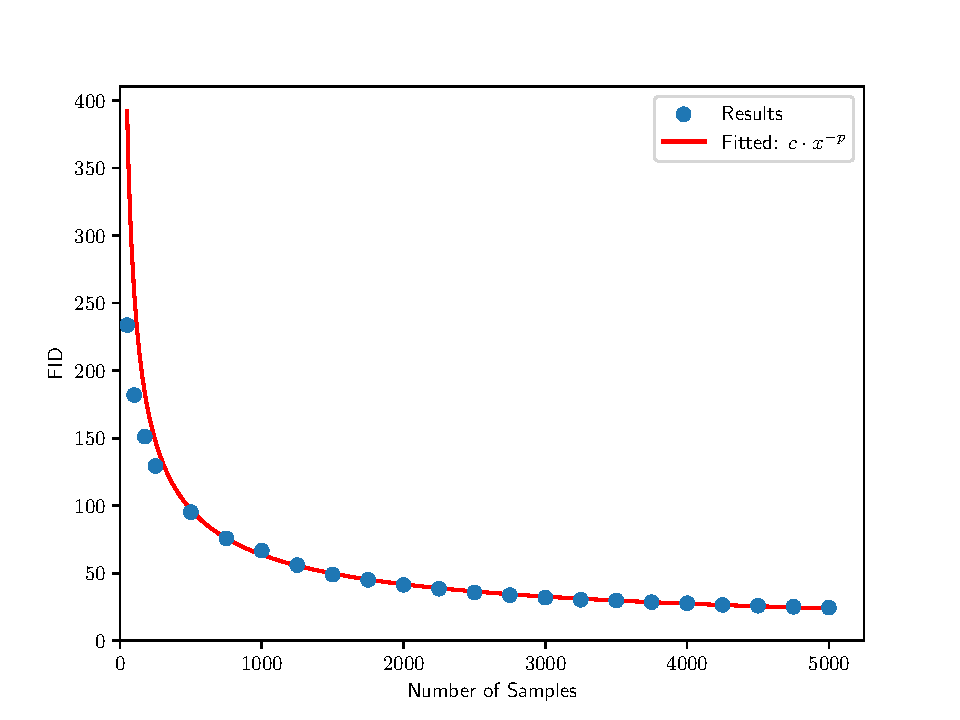
\includegraphics[width=\textwidth]{assets/num_samples_comparison.pdf}
        \caption{FID scores for datasets in different sizes.}
        \label{fig:num_samples_comparison}
    \end{subfigure}
    \hfill
    % Second subfigure: The PDF file 'num_samples_comparison_corrected.pdf'
    \begin{subfigure}{0.4\textwidth}
        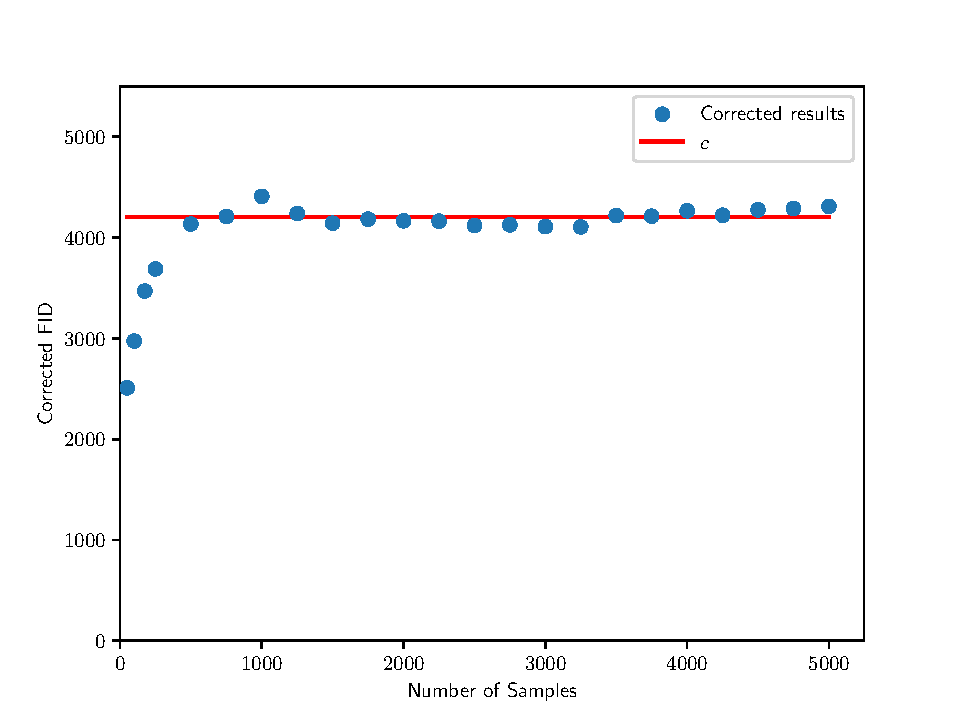
\includegraphics[width=\textwidth]{assets/num_samples_comparison_corrected.pdf}
        \caption{Graph of proposed corrected FID score.}
        \label{fig:num_samples_comparison_corrected}
    \end{subfigure}
    \caption{Comparison of FID scores across different sample sizes. Here, subsets of MS-COCO where used with 250 diffusion steps.}
\end{figure}

In general, we found the TID score to be very unstable. It can only be compared between models, where all the calculation and pipeline steps are exactly the same. To illustrate this phenomenon, we calculated the FID for different numbers of samples. The MS-COCO validation dataset, has 5000 images. We took subsets of this dataset in various sizes and computed the FID score again just as described on top. The results can be seen in fig. \ref{fig:num_samples_comparison}. As you can see, there is a consistent downwards trend, which indicates that the more samples exists in a given dataset, the better the TID score is. This happens because the FID score measures the difference between two feature distribution. With fewer data points, this difference is more susceptible for outliers, which increases the calculated difference. We would like to highlight that the FID is not only less accurate with fewer data points but simply worse.

As you can see in fig \ref{fig:num_samples_comparison}, the downwards trend inherits a predictable pattern. By linear regression of the log-log-plot, we were able to match the function
$$ y(x) = c\cdot \frac{1}{x^p} \qquad\mathrm{with}\quad p = 0.607,\, c = 4208.3$$
onto our data points. Equipped with this knowledge, we are able to propose a corrected FID score, by multiplying the FID score with the number of samples, the score was calculated with, to the $(-p)$-th power. The results can be viewed in fig. \ref{fig:num_samples_comparison_corrected}. This correction enables us to compare FID scores of different dataset sizes and also yields to the more desirable behavior, that the FID score is just less accurate for lower sample sizes and not straight up greater. 

There are clear open question, that require more research. $p$ and $c$ might depend on the dataset and/or the image-generating model, rendering the proposed correction useless. On the other hand, if at least $p$ is a global value for the FID score in general, this method makes FID scores of datasets of different sizes comparable. Maybe there is even a the

We were also interested in the FID score when varying the number of diffusion steps. As we didn't have the computation power, to generate 5000 images per number of diffusion steps, we only used a subset of 1780 images of the MS-COCO dataset. We consider the FID calculation with more than 1750 images a sufficiently stable – at least in our case – as from there on the corrected FID is roughly constant (Fig. \ref{fig:num_samples_comparison_corrected}). The results can be seen in \ref{fig:ddms_comparison}.
\begin{figure}[h]
    \centering
	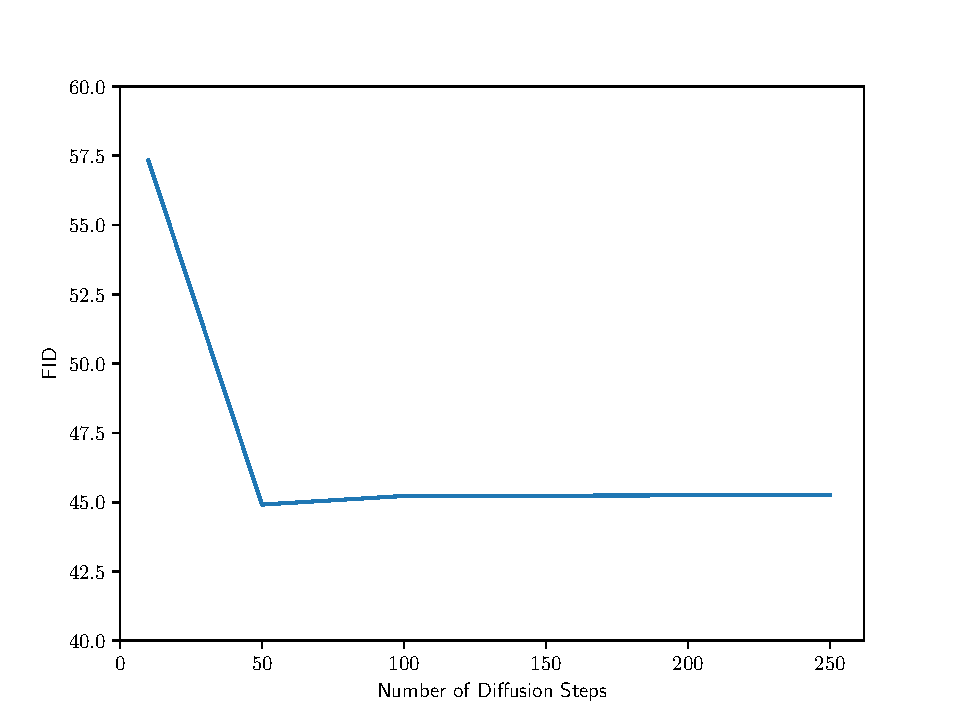
\includegraphics[width=0.4\textwidth]{assets/ddms_comparison.pdf}
	\caption{FID score by number of diffusion step for a subset of MS-COCO of size 1750.}
	\label{fig:ddms_comparison}
\end{figure}

As you can see, the FID score already settles at 50 diffusion steps, indicating constant quality from there on out. In fig. \ref{fig:ddms_image_comparison} you can make up your own mind. There we compared the different generated images for different prompts.

\begin{figure}[h!]
    \centering
	\includegraphics[width=0.85\textwidth]{assets/ddms_image_comparison.pdf}
	\caption{Generated images with different numbers of diffusion steps. On the right, the reference image from the MS-COCO dataset. The prompts where (1) \textit{A woman standing on skiis while posing for the camera.} (2) \textit{Suitcase sitting on the ground with stickers from various countries on it.} (3) \textit{Black and white photo of a scooter carrying numerous bikes.} (4) \textit{A corner of a kitchen with a big fridge.} (5) \textit{A small elephant walks underneath a big elephant.}} 
	\label{fig:ddms_image_comparison}
\end{figure}


\newpage

\section{Societal Impacts}
The capabilities the mentioned text-to-image models are already extraordinary, but development has not stopped with Würstchen. The quality of image generation was further improved\cite{lin2023designbenchexploringbenchmarkingdalle} and other capabilities where added in so-called multimodal models\cite{yasunaga2022retrievalaugmentedmultimodellanguagemodeling}. With this powerful new technology existing, one might immediately ask where these text-to-image models are used nowadays and what side effects does their usage have on different groups of people.

\subsection{Application in professional contexts}
The most self-evident influence might be on those working as professional artists. In 2023 Researchers in Korea conducted a survey on 28 professionals working in a wide variety of domains in the artistic sector, from sculpturing to video editing\cite{ko2023largescaletexttoimagegenartionmodelsforvisualartists}. 12 of them mentioned, that Stable Diffusion and its descendants are useful in generating more reference material, which they mainly use to learn by observing what and how others create and to get inspirations for new ideas. But most of them also stated, that, this wouldn't change their basic work paradigm. Another use case for them was rapid prototyping, in order to enable them to do real-time communication to their clients or artists in different fields. Furthermore, the artists perceived that the models have close to no bias when creating art, which made it possible to quickly create unconventional images but also yields the lack of the ability to personalize the results. They also said that because the generated images are only influenced by the text prompt and text can never fully and accurately describe and image the artist have in mind, using text-to-image technology limits their creativity, and you cannot escape the restriction of the text prompt. Often times, this made it frustrating to use image generating AI in their daily work. Despite their flaws, text-to-image models are an ever-growing technology that support and will support professional artists and numerous ways.

Apart from artists, professionals in other fields are also string to use Stable Diffusion-like AI. Nowadays, it is easier than ever to create good to great images that you have in mind. The trend can be labeled as the "Democratization of Art". A Finish study on game industry professionals\cite{vimpari2023texttoimagegenerationaibygameprofessionals} titled "An Adapt-or-die Type of Situation" explores all kinds of different ways, this new technology impacts the industry. A lot of the participants were experiencing fundamental transformation of their role. Already a third of them were using it daily, another third weekly. Many of the participants, where similarly to the Korean artists using the AI mostly for prototyping and ideation. Also in architecture\cite{sekban2022artandarchtitecture} text-to-image models can be used to generate design alternatives, for instance making a design more energy efficient or sustainable. The education sector has also proven to be an area, where image generating AI can be applied\cite{vartiainen2023aiincraftseducation}. Here it is again used for ideation but also as way for children externalize their ideas and conceptions. Although it was also highlighted that using text-to-image models in the classroom yield multiple challenges, for instance the question on what to assess when marking a student's work, as a lot might have been done by the AI. Even in tourism, applications are possible. By a Chinese study\cite{miao2023aiintourism}, those AI tools have the chance improve the anticipation, on-site and recollection experience of tourists. 

What I have presented is just the peak of many professional applications of Stable Diffusion and its decedents and I did not yet start with the private use cases. In general, we were able to make out, three major applications: final image creation, ideation and prototyping.

\subsection{Risks and Concerns}
Despite all those great opportunities and application, it is irrefutable that there are risks and negative impacts of the boom of this technology. 

As it is easier than ever to create convincing images, deepfakes become a big problem. At 22nd March 2023, a twitter post went viral claiming there has been an explosion at new Pentagon in Washington DC. The post included an AI generated image. The fake news was allegedly spread by among others by the Russian broadcast "Russia Today"\cite{correctiv2023pentagonexplosion} post like these are becoming more realistic and easier to produce. S. Neupane and other researcher from Mississippi State University\cite{neupane2023impactsriskgenerativeai} classify misinformation as one of the five main new attack vectors leveraging artificial intelligence. 

A serous concern relates to biases, those models impose and the generated images. Generally speaking, image generating models can only reproduce, what they have seen in training. This means that underrepresented data, will also be reproduced rarely. This can have serious impacts. A study by Microsoft\cite{naik2023socialbiasesthroughtexttoimage} showed that 70\% of the generated persons by Stable Diffusion were white. Also, woman are either largely underrepresented or overrepresented, most likely in order of circumvent this problem. One other notable finding was that when generating images to the prompt  "Office in Ethiopia", DALL-E and Stable Diffusion both depict Ethiopia as being in a state of poor economic conditions, while when actually looking for real images, they are closer to offices you might see in western countries. 

Further consequences of the underrepresentation of the Global South are usability issues. In a cooperation of computer scientists from US, Canada and Bangladesh\cite{mim2024impactoftexttoimagetoolsinglobalsouth}, a survey of Bangladeshi image practitioners was conducted. It was found that Bangladeshi had problems creating the text prompts. Citing one of their participants \textit{"Text-based prompts need proficiency in English nouns and adjectives to explain the idea of an image to the GAI [Generative AI] system to receive an outcome that matches the image practitioner's imagination."} Another participant complained, that specific Bangla words, do not have accurate English translation, in this case she wanted to describe a certain type of rain. Furthermore, often times the participants are poorly educated, such that, even if text-prompts were possible in their mother tong, they wouldn't be able to accurately articulate their perception of the image. Even worse, most of the participants rely on the usage of the free image generating technology, as traditional, more professional applications like \textit{Adobe Photoshop} or \textit{Adobe Illustrator} or financially not feasible. Also in this study impacts of the underrepresentation of data from the global south were found. They asked Midjourney, to depict a future version of Gawsia market, which resulted in an image, where neither the architectural characteristics nor the physical appearances of the people match those typically whitnisable in Dhaka.

Moving again to the Western world, especially when using generated images in commercial contexts, one question that has not been answered yet, is the question of copyright. To whom does a generated image belong? There are many possible answers: The artists, who created the training data, the company, who trained the text-to-image model, or the user, who created the text prompt. Currently, there are numerous lawsuits conducted on this topic. Most relevantly, Getty Images (a leading global stock photography and media company) has brought Stability AI (the company behind Stable Diffusion) to court accusing it of unlawfully using millions of its copyrighted images to train Stable Diffusion models without permission\cite{cnn2023gettyimagesvsstabilityai}.

\subsection{Conclusion}

The rapid advancements in text-to-image models, such as those exemplified by Würstchen and its successors, have had profound effects across various sectors. These models contributed to professional fields such as art, architecture, education, and tourism with valuable applications that enabled new ways of ideation, prototyping, and final image creation. Perhaps what is most important in the creative industries—making art democratized, now more people can create high-quality images easily—is a tectonic shift in creative industries, empowering professionals and amateurs alike.

These benefits are joined by major risks and challenges whereby deepfakes, bias reinforcement in generated content, and underrepresentation of the Global South in training data raise a number of ethical and practical concerns. More than that, vagueness over the question of copyright ownership with AI image generation adds legal headaches yet to be sorted.

It's crucial to address these issues in the future to maximize the benefits and minimize the harms as text-to-image technology evolves. Ongoing research, ethical considerations, and legal frameworks will shape the positive and negative impacts of this powerful technology on society.

\section{Discussion}
1.5 - 2 Seiten. Eigene meinung, auch über aktuelle Entwicklung

\newpage
\bibliographystyle{plain}
\bibliography{references}


\end{document}
